%%%%%%%%%%%%%%%%%%%%%%%%%%%%%%%%%%%%%%%%%%%%%%%%%%%%%%%%%%%%
%%  This Beamer template was created to be a simple and clean.
%%  Anyone can freely use or modify it for any purpose without
%%  attribution.
%%
%%  The starting point for this template was [1] with further
%%  inspiration from [2].  Logo taken from [3].
%%
%%  [1] http://cameron.bracken.bz/beamer-template
%%  [2] https://sites.google.com/a/umn.edu/jwolfson/tricks-templates
%%  [3] www.ur.umn.edu/brand/
%%
%%  Last Modified: August 27, 2014
%%  Hamid M.

\documentclass[xcolor=x11names,compress]{beamer}

%% General document %%%%%%%%%%%%%%%%%%%%%%%%%%%%%%%%%%
\usepackage{graphicx}
\usepackage{tikz}
\usepackage{verbatim}
\graphicspath{ {../images/} }
%%%%%%%%%%%%%%%%%%%%%%%%%%%%%%%%%%%%%%%%%%%%%%%%%%%%%%

% Define the ``official'' UMN colors
\xdefinecolor{GopherMaroon}{HTML}{7A0019}
\xdefinecolor{GopherGold}{HTML}{FFCC33}
\xdefinecolor{GopherLightGold}{HTML}{FFDE7A}
\xdefinecolor{GopherDarkMaroon}{HTML}{5B0013}


%% Beamer Layout %%%%%%%%%%%%%%%%%%%%%%%%%%%%%%%%%%
% Two Options, uncomment the desired option.
%   # 1: Navigation bar shows one 'bullet' per slide
\useoutertheme[subsection=false,shadow]{miniframes}
%%%% end of # 1

%   # 2: Navigation bar shows one bullet per subsection
%        Reference: http://tex.stackexchange.com/a/64419/60315
%\useoutertheme[subsection=false]{miniframes}
%\usepackage{etoolbox}
%\makeatletter
%\patchcmd{\slideentry}{\advance\beamer@xpos by1\relax}{}{}{}
%\def\beamer@subsectionentry#1#2#3#4#5{\advance\beamer@xpos by1\relax}%
%\makeatother
%%%% end of # 2

\linespread{1.5}
\usepackage{natbib}
\usepackage{bibentry}
\bibliographystyle{apalike}

\useinnertheme{default}
\usefonttheme{serif}
\usepackage{palatino}

\setbeamerfont{title like}{shape=\scshape}
\setbeamerfont{frametitle}{shape=\scshape}

\setbeamercolor*{lower separation line head}{bg=GopherMaroon} 
\setbeamercolor*{normal text}{fg=black,bg=white} 
\setbeamercolor*{alerted text}{fg=red} 
\setbeamercolor*{example text}{fg=black} 
\setbeamercolor*{structure}{fg=black} 
 
\setbeamercolor*{palette tertiary}{fg=GopherDarkMaroon,bg=GopherLightGold} 
\setbeamercolor*{palette quaternary}{fg=GopherDarkMaroon,bg=GopherLightGold} 
%%%%%%%%%%%%%%%%%%%%%%%%%%%%%%%%%%%%%%%%%%%%%%%%%%

% Customize template further %%%%%%%%%%%%%%%%%%%%%
% Add Logo and slide numbers to footer
\setbeamertemplate{footline}{\parbox{\textwidth}{\vspace*{-15pt}
                             ~~
                             
\includegraphics[width=0.25\paperwidth]{logoumn} 
                             \hfill 
                             \color{gray}{\tiny \insertframenumber\,/\,\inserttotalframenumber~~~}}}
\setbeamertemplate{navigation symbols}{}    % remove navigation symbols (http://tex.stackexchange.com/a/688)
%%%%%%%%%%%%%%%%%%%%%%%%%%%%%%%%%%%%%%%%%%%%%%%%%%


\begin{document}
\nobibliography*
%%%%%%%%%%%%%%%%%%%%%%%%%%%%%%%%%%%%%%%%%%%%%%%%%%%%%%
%%%%%%%%%%%%%%%%%%%%%%%%%%%%%%%%%%%%%%%%%%%%%%%%%%%%%%
\title{Indoor Micro-UAV Navigation with Minimal Sensing}
%\subtitle{SUBTITLE}
\author{
	Dennis Melamed\footnote{Dept. of Electrical and Computer Engineering}\\
	Advisers: Professor Volkan Isler\footnote{Dept. of Computer Science and Engineering} \& Professor Derya Aksaray\footnote{Dept. of Aerospace Engineering and Mechanics}\\
}
\date{\today}

{% no page #, no logo on title page
  \setbeamertemplate{footline}{}
  \begin{frame}
    \titlepage
  \end{frame}
}

%%%%%%%%%%%%%%%%%%%%%%%%%%%%%%%%%%%%%%%%%%%%%%%%%%%%%%
%%%%%%%%%%%%%%%%%%%%%%%%%%%%%%%%%%%%%%%%%%%%%%%%%%%%%%
\section{\scshape Overview}
\begin{frame}{Outline}
\tableofcontents
\end{frame}

%short blurb of what im doing
\begin{frame}{Proposed Project \& Success Criteria}
	\begin{itemize}
		\item Fly through door, land safely
		\item Random initial location
		\item Low-quality sensors \\(Camera, IMU)
		\item 27g weight
	\end{itemize}
	Success: Fly with $<$20\% failure rate through door (failure=crash, battery loss, missing door)\\
	\tiny{Source: \url{https://www.bitcraze.io/crazyflie-2/}}
	\begin{picture}(5.2, 3.4)
		\put(20,40){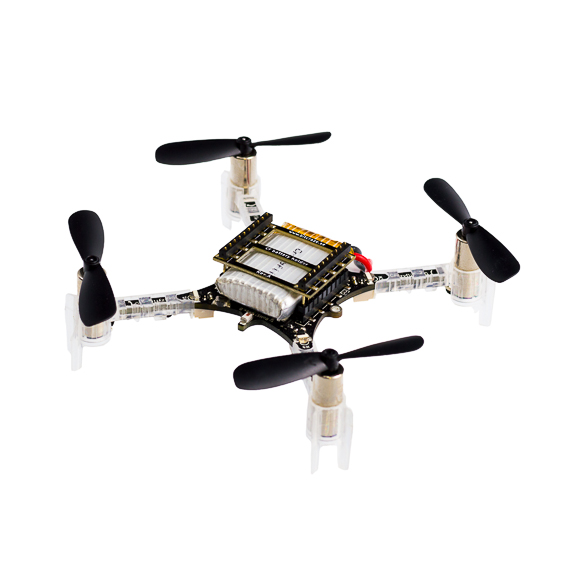
\includegraphics[scale=1]{crazyflie_new}}
	\end{picture}
\end{frame}

%%%%%%%%%%%%%%%%%%%%%%%%%%%%%%%%%%%%%%%%%%%%%%%%%%%%%%
%%%%%%%%%%%%%%%%%%%%%%%%%%%%%%%%%%%%%%%%%%%%%%%%%%%%%%
\section{\scshape Background}

%why necessary
%gapflyt
%flying indoors
%crazyflie size comparison
\begin{frame}{Background}
	\vspace{-40pt}
	\begin{itemize}
		\item Research with autonomous navigation\\
			in constrained spaces 
		\begin{itemize}
			\item GapFlyt 
		\end{itemize}
		\item Research with small scale UAV control\\
			in motion capture systems
		\begin{itemize}
			\item Morphing
		\end{itemize}
		\item Combination not well studied
	\end{itemize}
	\begin{picture}(5.2, 3.4)
		\put(220,20){\includegraphics[scale=0.05]{gapflyt}}
	\end{picture}
	\begin{picture}(5.2, 3.4)
		\put(80,-60){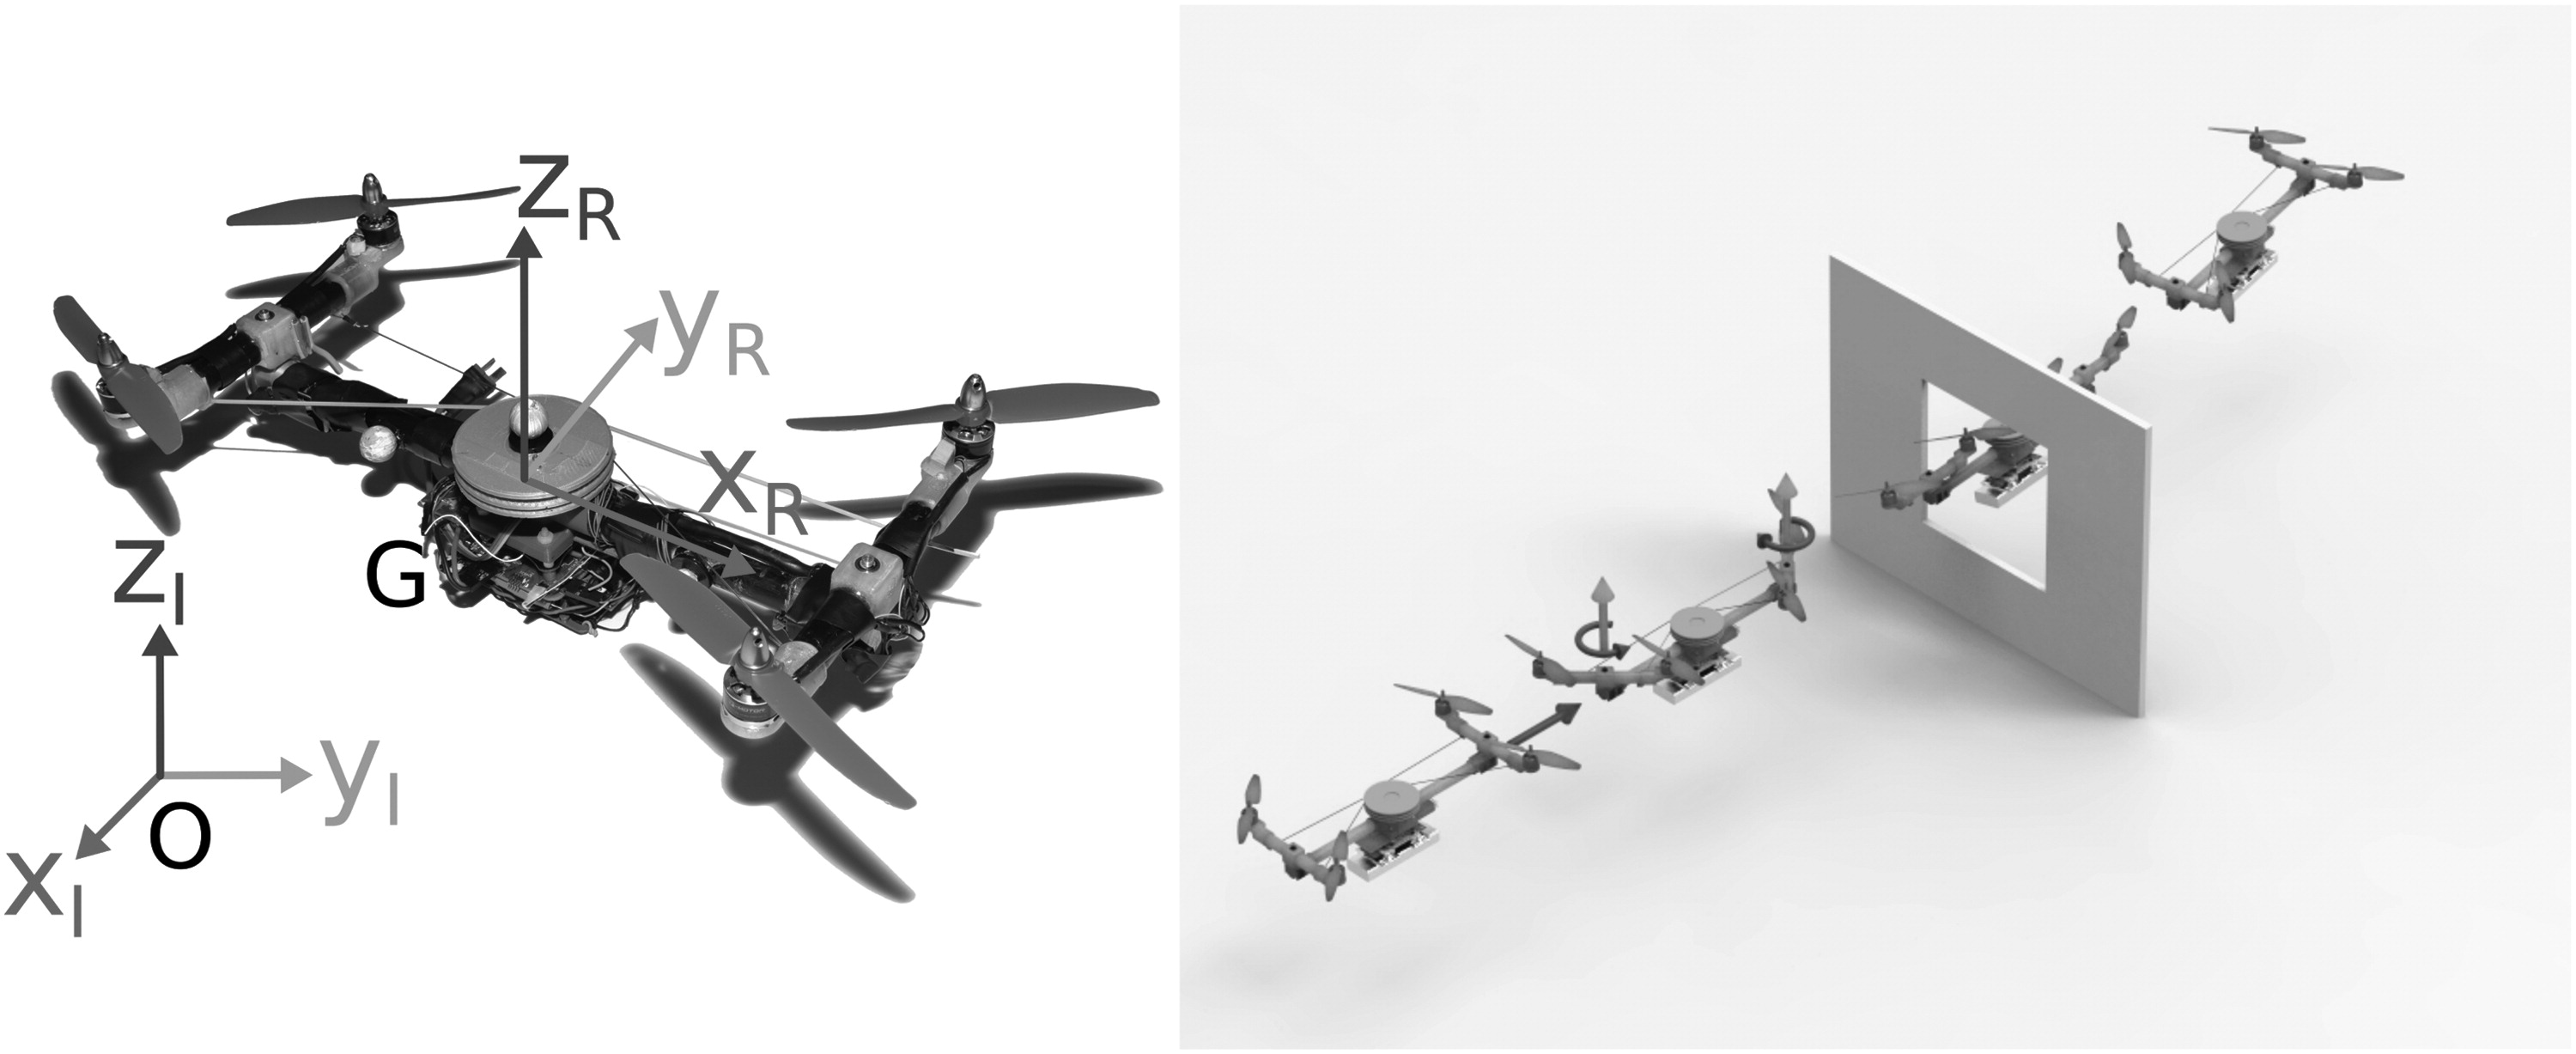
\includegraphics[scale=0.5]{morphing}}
	\end{picture}
	\tiny{Source: \\\cite{gapflyt}\\ \cite{Folding}}
\end{frame}


%%%%%%%%%%%%%%%%%%%%%%%%%%%%%%%%%%%%%%%%%%%%%%%%%%%%%%
%%%%%%%%%%%%%%%%%%%%%%%%%%%%%%%%%%%%%%%%%%%%%%%%%%%%%%
\section{\scshape Methodology}



\begin{frame}{Project Overview}
	\vspace{-10pt}
	\begin{itemize}
		\item Initial setup
		\begin{itemize}
			\item Motion capture
		\end{itemize}
		\item Door detection
		\item Independent Flight
	\end{itemize}
\end{frame}

\subsection{Door Detection}

\begin{frame}{Door Detection - Hough Transform}
	\begin{itemize}
		\item Hough Transform for line detection	
		\item Group close-to-parallel lines
		\item Choose largest rectangle formed
	\end{itemize}
	\begin{picture}(5.2, 3.4)
		\put(200,10){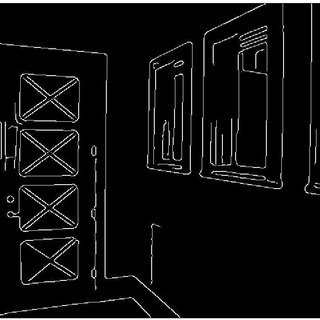
\includegraphics[scale=0.5]{canny_edge}}
		\tiny{Source: \cite{parallelogram}}
	\end{picture}
\end{frame}

\begin{frame}{Door Detection - Fuzzy Logic}
	\begin{itemize}
		\item Fuzzy concept of vertical/horizontal line
		\item Fuzzy concept of door frame (2 vertical + 1 horizontal)
	\end{itemize}
	\cite{Fuzzy}
\end{frame}

\begin{frame}{Door Detection - Fully Convolutional Neural Network}
	\begin{itemize}
		\item Add noise/lower resolution
		\item Output segmented door
	\end{itemize}
$$
IoU = \frac{AreaOfOverlapBetweenDetections}{AreaOfUnionOfDetections}
$$	
	\begin{picture}(5.2, 3.4)
		\put(200,60){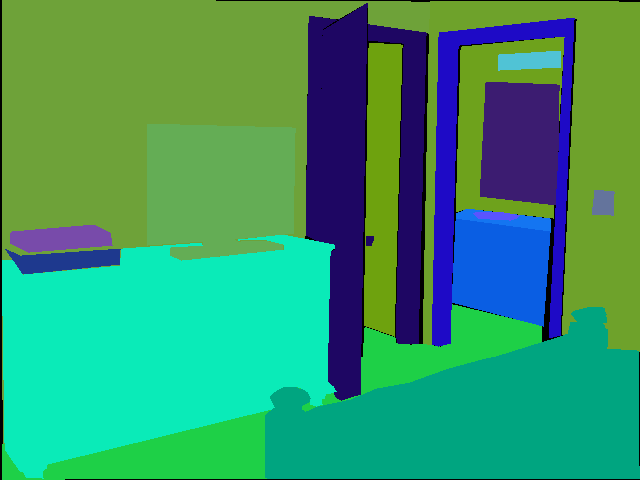
\includegraphics[scale=0.20]{door_csail}}
		\tiny{Source: \cite{csail_data_1}}
	\end{picture}
\end{frame}

\subsection{Independent Flight}
\begin{frame}{Independent Flight - Dead Reckoning}
	\begin{itemize}
		\item Calculation of unit vector pointing at door
		\item Launch and fly quickly to minimize drift
	\end{itemize}
\end{frame}

\begin{frame}{Independent Flight - Recurrent Neural Network}
	\begin{itemize}
		\item Train network w/ waypoint navigation ground truth
		\item Has memory - deal with velocities
	\end{itemize}
\end{frame}

\begin{frame}{Independent Flight - Reinforcement Learning}
	\begin{itemize}
		\item Similar inputs/outputs as regular RNN
		\item Train without ground truth, reward instead:
		\begin{itemize}
			\item $D$ - distance from door
			\item $R$ - is UAV orientation acceptable
			\item $O$ - distance to obstacles
		\end{itemize}

$$
Reward = K_{1}/D + K_{2}*R + K_{3}*O + K_{n}*OtherFactors
$$
	\end{itemize}
\end{frame}

\section{\scshape Conclusion}

\begin{frame}{Budget \& Schedule}
	\begin{itemize}
		\item Small budget for wood to build door (~\$20)
		\item Oct 25 - Initial setup and UAV flight
		\item Dec 12 - Door detection algorithms compared
		\item Apr 05 - Independent flight algorithms compared
	\end{itemize}
\end{frame}

\begin{frame}{Conclusion}
	\vspace{-60pt}
	\begin{itemize}
		\item Explore intersection of small size, auto navigation
		\item Compare methods for door detection
		\item Compare methods for independent flight
	\end{itemize}
	\begin{picture}(5.2, 3.4)
		\put(0,-80){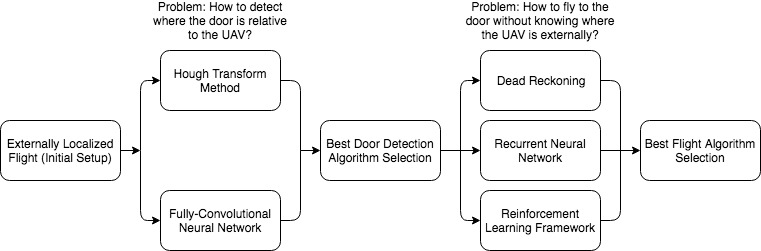
\includegraphics[scale=0.4]{flowchart}}
	\end{picture}
\end{frame}

\begin{frame}
	Questions
\end{frame}

\begin{frame}{References}
	\tiny{\bibliography{../references}}
\end{frame}

\begin{frame}{Simulation}
	\begin{itemize}
		\item Virtual Robotics Experimentation Platform (VREP)
		\item Input/Output same form as real Crazyflie
		\item Noisy, low resolution camera
		\item Noise IMU
		\item Delay to mimic data down-link
	\end{itemize}
\end{frame}

\begin{frame}{Motion Capture}
	\begin{itemize}
		\item VICON
		\item Set of cameras
		\item Track balls on desired object
		\item Provide orientation/position but only w/i tracked space
		\item Safety net: bad UAV orientation/path = shut down
	\end{itemize}
	\begin{picture}(5.2, 3.4)
		\put(120,90){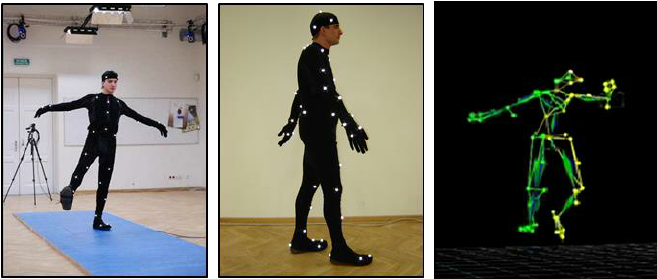
\includegraphics[scale=0.3]{mocap}}
		\tiny{Source: \cite{mocap}}
	\end{picture}

\end{frame}

\begin{frame}{Hough Transform}
	\begin{itemize}
		\item Edge detector
		\item Parametrize line:
		\item $r = x*cos(\theta) + y*sin(\theta)$
		\item For each edge point: determine all $r$, $\theta$ solving above, increment table
		\item Maximums of table give lines majority of points agree on 
	\end{itemize}
	\begin{tikzpicture}[scale=1]
	    % Draw axes
	    \draw [<->,thick] (0,2) node (yaxis) [above] {$\theta$}
		|- (3,0) node (xaxis) [right] {$r$};
	\end{tikzpicture}
	\vspace{10pt}

\end{frame}



\end{document}
